\chapter{Solución Propuesta}
\label{chap-solution}

En esta Sección se describen las técnicas aplicadas para lograr el seguimiento
de los jugadores. En primer lugar, se detallan algoritmos utilizados para
ignorar los elementos del fondo de la imagen en la Sección
\ref{sec:background-elimination}. Luego, se detalla cómo fue utilizado el
algoritmo contornos activos y las modificaciones que se le hicieron en la
Sección \ref{sec:ac-extension}.

\section{Eliminación de Fondo}

\label{sec:background-elimination}
Se evaluó que el análisis por contornos activos se beneficiaría de un análisis
previo que detecte y otorga información al proceso de actualización de
contornos activos sobre qué sectores de los cuadros del video no corresponden a
las siluetas de los objetos de interés para el seguimiento.

Con ese fin, se analizaron distintos métodos para extraer información adicional
de la imagen y detectar e ignorar sectores de la imagen que no correspondan a
jugadores. A continuación se describen los métodos evaluados.

\subsection{Tribuna y Publicidades}
\label{subsec:crop-tribunas}

La técnica más simple de eliminación de sectores es una técnica de
\textit{recorte} que elimina de la imagen todo píxel ajeno a un polígono
(como ser un cuadrilátero) que bordea la cancha. En las Figuras
\ref{fig:crop-antes} y \ref{fig:crop-despues} se muestra el resultado de
aplicar esta técnica a uno de los videos utilizados.

\begin{figure}[H]
  \centering
    \begin{minipage}[t]{.45\textwidth}
      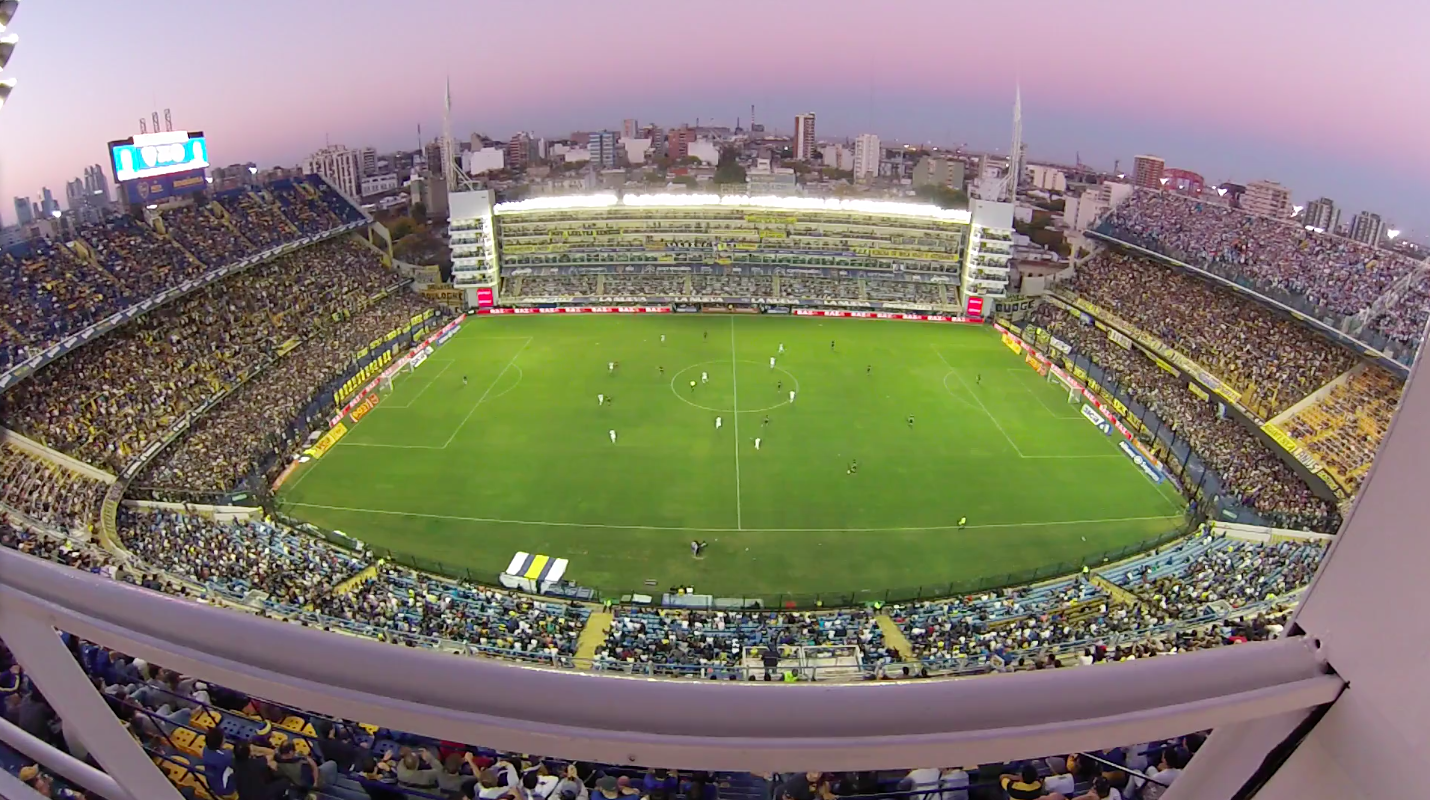
\includegraphics[width=\linewidth]{./images/Crop_Antes.png}
      \caption{Un cuadro del video de un partido.
      \label{fig:crop-antes}}
    \end{minipage}
    \begin{minipage}[t]{.45\textwidth}
      \centering
      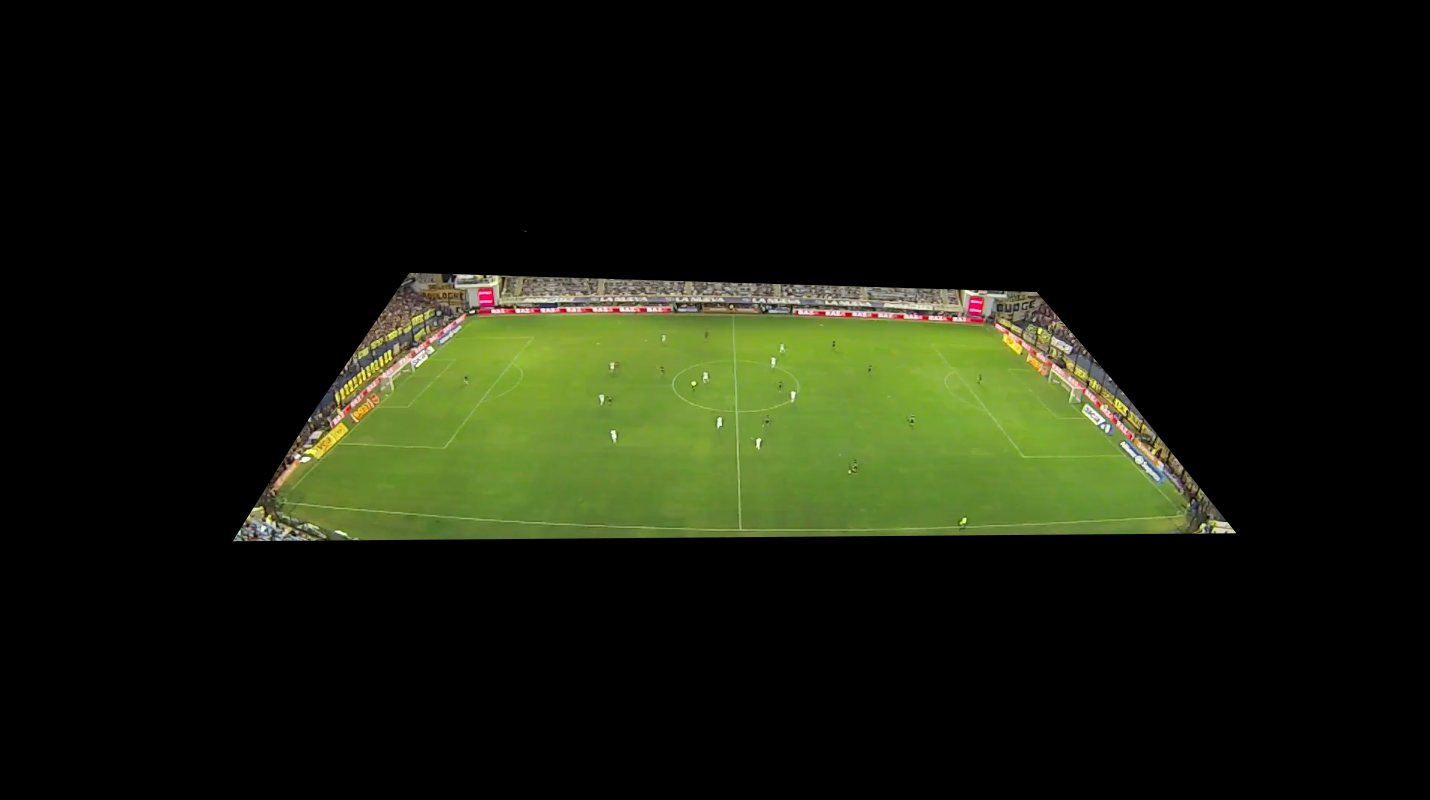
\includegraphics[width=\linewidth]{./images/Crop_Despues.png}
      \caption{El mismo cuadro, luego de aplicar la operación \textit{recorte}.
      \label{fig:crop-despues}}
    \end{minipage}
\end{figure}

\subsection{Substracción de Fondo por Valor de Energía}

Se implementó el método de eliminación de fondo descripto en
\cite{papers-tanos} para eliminación de sectores que corresponden al verde del
césped de la cancha o las líneas blancas pintadas sobre el mismo, basado en una
medición de la variación del color de cada píxel, a la cual se refiere como
energía.

Este no resultó ser un método apropiado debido a que el sistema de codificación
del video genera muchos falsos negativos, sobre todo \textit{glitches}. Un
\textit{glitch} es un error (de encodificación o filmación) que genera cambios
en los valores de colores (aumentando la energía de ese píxel). La gran
cantidad de \textit{glitches} alrededor de las líneas de la cancha les otorga a
estos puntos un mayor valor de energía del que realmente tienen. En la Figura
\ref{fig:tanos-fondo-sin} se muestra un recorte del primer cuadro del video de
un partido entre Boca e Independiente. En las figuras \ref{fig:tanos-fondo} y
\ref{fig:tanos-fondo-broken} se muestra el resultado de aplicar este algoritmo
en ese mismo recorte. Se puede ver que en el cuadro \#27 detecta muy bien el
fondo, pero los cambios que se producen en el cuadro siguiente confunden al
método, eliminando algunos píxels que estaban bien detectados.

\begin{figure}[H]
  \centering
    \begin{minipage}[t]{.45\textwidth}
      
\includegraphics[width=\linewidth]{./images/tanos-fondo-f1.png}
      \caption{Recorte del cuadro \#1 del video del partido entre Boca e Independiente
      \label{fig:tanos-fondo-sin}}
    \end{minipage}
    \begin{minipage}[t]{.45\textwidth}
      
\includegraphics[width=\linewidth]{./images/tanos-fondo-f27.png}
      \caption{Recorte del cuadro \#27 del video. El color azul denota los píxeles detectados como fondo por el algoritmo.
      \label{fig:tanos-fondo}}
    \end{minipage}
  \end{figure}
  \begin{figure}[H]
  \centering
    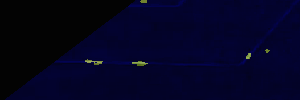
\includegraphics[width=.45\linewidth]{./images/tanos-fondo-f28.png}
    \caption{Recorte del cuadro \#28 del video. En este caso, el efecto de \textit{glitch} causa un falso negativo y no detecta parte de la cancha como fondo.}
    \label{fig:tanos-fondo-broken}
\end{figure}

Otro problema encontrado con este algoritmo es que, al basarse en cambios de color,
puede considerar que un jugador que se encuentra estático durante varios cuadros
es parte de fondo. Si bien los jugadores suelen estar en movimiendo durante el
partido, esto no es tan cierto en el caso del arquero.

Por los motivos detallados, se descartó el uso de este algoritmo en favor de las
técnicas descriptas en la próximas Secciones, \ref{sec:lineas} y \ref{sec:cesped}.

\subsection{Eliminación de Líneas}
\label{sec:lineas}

Las líneas blancas que delimitan la cancha y sus distintas partes presentan un
problema para el seguimiento de los equipos con camisetas blancas o de colores
claros. Para evitar que el algoritmo de contornos activos considere que las
líneas son parte de un jugador, como en la figura \ref{fig:confusion-linea}, se
considera otro método para detectarlas e ignorar estos puntos al momento de
realizar el paso de actualización de contornos.

Se desarrolló un método similar que detecta los tramos pintados de blanco en el
césped de la cancha. El mismo funciona aplicando un detector de bordes (se
utilizaron tanto el método de Roberts como el de Canny), umbralizando el
resultado, y haciendo un análisis morfológico de las componentes conexas
obtenidas luego de la umbralización.  Este método está basado en la idea detrás
del algoritmo de detección de líneas de Hough.

El análisis morfológico considera que una componente conexa entre píxeles
detectados como bordes es un jugador si se cumplen las siguientes condiciones:
\begin{itemize}
  \item El ancho de la región es menor a un valor de umbral $M_{width}$.
  \item El alto de la región es menor a un valor de umbral $M_{height}$.
  \item El área cubierta es menor a un valor de umbral $M_{area}$.
\end{itemize}

Estos tres valores son parámetros del algoritmo y dependen de la resolución y
\textit{zoom} del video (a mayor resolución, los jugadores abarcan mayor área y
las regiones que ocupan son más altas y anchas).

\begin{figure}[H]
  \centering
  
\includegraphics[width=0.3\linewidth]{./images/confusion-linea.png}
  \caption{ Resultado de aplicar el algoritmo sin eliminación de líneas.
    El color celeste delimita el contorno de un jugador, incluyendo erróneamente
    parte de las lineas de la cancha.}
      \label{fig:confusion-linea}
\end{figure}

\subsection{Eliminación del Césped}
\label{sec:cesped}

Para la eliminación del césped del campo de juego se requiere caracterizar los
píxeles correspondientes al verde del campo. Para esto, se realiza un análisis
de los colores de la imagen recortada, es decir la imagen resultante luego
aplicar la técnica de \textit{recorte}, detallada en
\ref{subsec:crop-tribunas}, una vez seleccionados los contornos iniciales de
los jugadores. El análisis consta de calcular el valor promedio y desvío
estándar del conjunto de píxeles que no forme parte de los jugadores o un
elemento ya conocido del fondo (por ejemplo, las líneas de la cancha sobre el
césped).

Con este valor, se considera parte del césped cualquier punto que no tenga las
características de un jugador (según definidas en la Sección
\ref{sec:caracteristicas}), y se encuentre a menos de $3$ desvíos del color
promedio calculado.

\section{Contornos activos} \label{sec:ac-extension}

\textit{Contornos Activos} requiere para su implementación que se definan dos
funciones. Una es la función de probabilidad $p$ y la otra la función
característica $v$ (ver Sección \ref{sec:ac}). En esta Sección se describe la
elección de ambas funciones para este trabajo.

\subsection{Características}
\label{sec:caracteristicas}

Como se explica en la Sección \ref{sec:ac-problemas}, cuando los objetos de
interés son complejos, la utilización del color promedio como única
característica distintiva no alcanza. Es por esto que varias de las mejoras
planteadas al algoritmo de contornos activos giran en torno a la selección de
características para representar a los objetos de interés. A continuación, se
describen los cambios que se han incorporado para hacer el algoritmo más
efectivo ante un video correspondiente a un partido de fútbol.

Si bien el color promedio resulta insuficiente para caracterizar correctamente
al objeto, puede utilizarse en complemento con otras características. Una opción
es la utilización del desvío estándar de color en el objeto de interés.
Este se calcula de la manera descripta en el Algoritmo \ref{alg:desvio},
donde la rutina \textit{DesvioLocal} se define en el Algoritmo \ref{alg:desvio-local}.

\begin{algorithm}
    \caption{Característica Desvío Estándar}
    \label{alg:desvio}
    \begin{algorithmic}
    \Require\hspace{\algorithmicindent}\hspace{\algorithmicindent}Cuadro c, Contornos $\omega_1 \dots \omega_n$

    \Ensure\hspace{\algorithmicindent}\hspace{0.23cm} $(r_{dev}, g_{dev}, b_{dev})$
    \State

    \State $\Omega \gets \cap \omega_1 \dots \omega_n$
    \State $count \gets 0$
    \State $r_{sum} \gets 0$
    \State $g_{sum} \gets 0$
    \State $b_{sum} \gets 0$
    \For{$p \in c$}

        \If{$p \not\in  \Omega$}
            \State $count \gets count + 1$
            \State $(r_{dev}, g_{dev}, b_{dev}) \gets $ DesvioLocal($p, c$)
            \State $r_{sum} \gets r_{dev} + r_{sum}$
            \State $g_{sum} \gets g_{dev} + g_{sum}$
            \State $b_{sum} \gets b_{dev} + b_{sum}$
        \EndIf
    \EndFor

    \State \Return $ (\frac{r_{sum}}{count}, \frac{g_{sum}}{count}, \frac{b_{sum}}{count}) $
    \end{algorithmic}
\end{algorithm}

\begin{algorithm}[H]
    \caption{DesvioLocal}
    \label{alg:desvio-local}
    \begin{algorithmic}
    \Require\hspace{\algorithmicindent}\hspace{\algorithmicindent}Posición $p$, Cuadro c,
    \Ensure\hspace{\algorithmicindent}\hspace{0.23cm} $(r_{dev}, g_{dev}, b_{dev})$
    \State

    \State $r_{avg} \gets 0$
    \State $g_{avg} \gets 0$
    \State $b_{avg} \gets 0$
    \For{$p'$ 8-conectado a $p$}
        \State $(r, g, b) \gets c_{p'}$
        \State $r_{avg} \gets r + r_{avg}$
        \State $g_{avg} \gets g + g_{avg}$
        \State $b_{avg} \gets b + b_{avg}$
    \EndFor

    \State $(r_{avg}, g_{avg}, b_{avg}) \gets (\frac{r_{sum}}{count}, \frac{g_{sum}}{count}, \frac{b_{sum}}{count}) $

    \State $r_{dev} \gets 0$
    \State $g_{dev} \gets 0$
    \State $b_{dev} \gets 0$
    \For{$p'$ 8-conectado a $p$}
        \State $(r, g, b) \gets c_{p'}$
        \State $r_{dev} \gets r_{dev} + (r - r_{avg})^2$
        \State $g_{dev} \gets g_{dev} + (g - g_{avg})^2$
        \State $b_{dev} \gets b_{dev} + (b - b_{avg})^2$
    \EndFor

    \State \Return $ (\sqrt{\frac{r_{dev}}{8}}, \sqrt{\frac{g_{dev}}{8}}, \sqrt{\frac{b_{dev}}{8}}) $

    \end{algorithmic}
\end{algorithm}

Entonces la función $v$ queda defininida como:

\begin{eqnarray*}
    (r, g, b) &=&  c_{x} \\
    (r_{dev}, g_{dev}, b_{dev}) &=& \text{DesvioLocal}(x, c) \\
    v(x) &=& (r, g, b, r_{dev}, g_{dev}, b_{dev})
    %v(p) = (r_{avg}, g_{avg}, b_{avg}, r_{dev}, g_{dev}, b_{dev})
\end{eqnarray*}

Y para cada contorno se define su vector característico $v_i$ como el resultado de aplicar
los Algoritmos \ref{alg:carac-rgb} y \ref{alg:desvio}.

\begin{algorithm}
    \caption{PromedioRGB}
    \label{alg:carac-rgb}
    \begin{algorithmic}
    \Require\hspace{\algorithmicindent}\hspace{\algorithmicindent}Cuadro c, Contorno $\omega$

    \Ensure\hspace{\algorithmicindent}\hspace{0.23cm} $(r_a, g_a, b_a)$
    \State

    \State $count \gets 0$
    \State $r_{sum} \gets 0$
    \State $g_{sum} \gets 0$
    \State $b_{sum} \gets 0$
    \For{$p \in \omega$}
        \State $count \gets count + 1$
        \State $(r, g, b) \gets c_{p}$
        \State $r_{sum} \gets r + r_{sum}$
        \State $g_{sum} \gets g + g_{sum}$
        \State $b_{sum} \gets b + b_{sum}$
    \EndFor

    \State \Return $ (\frac{r_{sum}}{count}, \frac{g_{sum}}{count}, \frac{b_{sum}}{count}) $
    \end{algorithmic}
\end{algorithm}


\subsubsection{Aprendizaje de valores}

Debido a que a lo largo del campo de juego la iluminación no es uniforme, y que
durante el partido la misma puede cambiar, se realiza un aprendizaje simple
de las características de cada contorno. En cada cuadro, siendo $\mathbf{v}$ un
vector con las características de un contorno dado, se calcula el promedio de
los valores de las características para todos los píxeles pertenecientes al
contorno y se lo denomina $\hat{\mathbf{v}}$. A continuación se actualiza
$\mathbf{v}$ y se lo reemplaza por un nuevo valor $\mathbf{v_n}$ calculado de
acuerdo a:

\[
  \mathbf{v_n} = \left(1-\alpha\right)\mathbf{v} + \alpha \hat{\mathbf{v}}
\]

Se toma un valor de $\alpha$ del orden de $10^{-2}$, es decir, se toma el $1\%$
de $\hat{\mathbf{v}}$. Esto evita la posibilidad de que se memoricen cambios
no deseados, como podría ser una oclusión parcial, antes de su correción.

\subsection{Función de Probabilidad}

Si bien la función de probabilidad sugerida en la Seccion \ref{sec:ac} se puede
aplicar en este caso, se modificó para tener en cuenta la morfología de los objetos
a seguir.

Se plantea que los jugadores estarán contenidos dentro de un rectángulo de
mayor altura que ancho. Se estima el máximo valor posible del ancho y alto de
un rectángulo que contenga a un jugador, y luego se limita el tamaño del
contorno, reduciendo la posibilidad de que el contorno se expanda por áreas
cuyos píxeles poseen características similares a las de píxeles que representan
a un jugador, pero como este área no cumple con la restricción de tener un
ancho o alto mayor al máximo permitido, se evita la expanción del contorno.
Dado que el algoritmo de contornos activos es utilizado en las líneas del
césped del campo de juego para evaluar si un punto pertenece al fondo o no, se
sugieren dos funciones de probabilidad, una denominada $f$ utilizada para la
detección del fondo y una función $f_j$ para el seguimiento de los jugadores,
definidas como:

\begin{eqnarray*}
    f(p) &=& 1 - \frac{\| v(p) - v_i \|}{255 * 6} \\
    f_j(p) &=& 1 - \min(1, f(p) + \text{distance\_weight}(p_x, p_y, \omega_i))
\end{eqnarray*}

Donde $v_i$ es el valor característico para el contorno $\omega_i$ contra el
que se evalua el punto $p$. Y la rutina \textit{distance\_weight} se define en
el Algoritmo \ref{alg:distance-weight}, donde $maxX$ y $maxY$ son el semi-ancho
y la semi-altura máxima del rectángulo, respectivamente.

\begin{algorithm}
    \caption{distance\_weight}
    \label{alg:distance-weight}
    \begin{algorithmic}
    \Require\hspace{\algorithmicindent}\hspace{\algorithmicindent}Posición $(x, y)$, Contorno $\omega$

    \Ensure\hspace{\algorithmicindent}\hspace{0.23cm} Un número
    \State

    \State $centroid_x \gets 0$
    \State $centroid_y \gets 0$
    \For{$p \in \omega$}
        \State $centroid_x \gets centroid_x + p_x$
        \State $centroid_y \gets centroid_y + p_y$
    \EndFor

    \State $centroid_x \gets \frac{centroid_x}{\#\omega}$
    \State $centroid_y \gets \frac{centroid_y}{\#\omega}$


    \State $res \gets 0$
    \State $dist_x \gets \|p_x - centroid_x\|$
    \State $dist_y \gets \|p_y - centroid_y\|$

    \If{$dist_x > max_x$}
        \State $res \gets res + \min(1, \frac{dist_x - max_x}{max_x})$
    \EndIf

    \If{$dist_y > max_y$}
        \State $res \gets res + \min(1, \frac{dist_y - max_y}{max_y})$
    \EndIf

    \State \Return $res$
    \end{algorithmic}
\end{algorithm}

\subsubsection{Seguimiento por Complemento}

% TODO: Esto estaba escrito feo, lo reescribí pero alguien que lo revise por las dudas
% Firma Esteban
Como es explicado en la Sección \ref{sec:ac-problemas}, no resulta evidente
cómo construir una función $v$ para camisetas que presenten más de un color. Si
bien el agregado del Desvío Estandard contribuye a mejorar el seguimiento en % TODO: Cómo contribuye?
estos casos, no soluciona totalmente el problema. Para poder seguir
correctamente a equipos cuyas camisetas presentan este desafio, se ofrece la
posibilidad de descartar el algoritmo de contornos activos para el seguimiento
de este equipo y determinar que los espacios que por sus características no son
definidos como césped, líneas de la cancha, o jugadores de otro equipo, son
jugadores del equipo cuyas características son difíciles de determinar. Este
método solo es efectivo si uno de los equipos puede ser correctamente
identificado por contornos activos.

Con este fin, se ejecuta el algoritmo de contornos activos sobre el primer
cuadro, con los jugadores del equipo identificable seleccionados. Luego, se
aplica el procedimiento \textit{complemento}, detallado en el Algoritmo
\ref{alg:complemento}. La salida de este procedimiento marca todo punto que no
fue identificado bajo ningún conjunto con el color \textit{cyan}, y aplica un
operador morfologico de expansión sobre todos estos puntos con el objeto
de unificar conjuntos que están cercanos.

\begin{algorithm}
    \caption{complemento}
    \label{alg:complemento}
    \begin{algorithmic}
    \Require\hspace{\algorithmicindent}\hspace{\algorithmicindent}Cuadro $c$, Contornos $\omega_1 \dots \omega_n$,
    cesped y lineas $\omega_0$

    \Ensure\hspace{\algorithmicindent}\hspace{0.23cm} Cuadro $c$
    \State

    \State $\Omega \gets \cap{\omega_0 \dots \omega_n}$
    \For{$(x, y) \in c$}
        \If{$(x, y) \not \in \Omega$}
            \State $c_{x, y} \gets \text{\textit{CYAN}}$

            \For{$(x', y') \text{4-conectado a} (x, y)$}
                \State $c_{x', y'} \gets \text{\textit{CYAN}}$
            \EndFor
        \EndIf
    \EndFor

    \State \Return $c$
    \end{algorithmic}
\end{algorithm}

Luego de esto, se utiliza la técnica de contornos activos siendo la función de
probabilidad de los contornos del segundo equipo una función que devuelve $1$
si el píxel es color \textit{cyan}, y $0$ en caso contrario.

